表 9 \textbar{} DeepSeek-V4-Pro 的智能体搜索与检索增强搜索对比。

{\def\LTcaptype{none} % do not increment counter
\begin{longtable}[]{@{}lllllllll@{}}
\toprule\noalign{}
\endhead
\bottomrule\noalign{}
\endlastfoot
Difficulty & Category & \# & Agent Win & RAG Win & Tie & Agent\% & RAG\%
& Tie\% \\
\multirow{2}{*}{Easy} & Objective Q\&A (客观问答) & 196 & 110 & 43 & 43
& 56.1 & 21.9 & 21.9 \\
& Subjective Q\&A (主观问答) & 321 & 198 & 56 & 67 & 61.7 & 17.4 &
20.9 \\
\multirow{2}{*}{Hard} & Objective Q\&A (客观问答) & 168 & 102 & 33 & 33
& 60.7 & 19.6 & 19.6 \\
& Subjective Q\&A (主观问答) & 184 & 126 & 27 & 31 & 68.5 & 14.7 &
16.8 \\
& Total (总计) & 869 & 536 & 159 & 174 & 61.7 & 18.3 & 20.0 \\
\end{longtable}
}

表 10 \textbar{} DeepSeek-V4-Pro 的成本对比：智能体搜索 vs.~检索增强搜索（均值）。在智能体搜索中，大多数工具调用是并行执行的。

{\def\LTcaptype{none} % do not increment counter
\begin{longtable}[]{@{}|l|l|l|l|@{}}
\toprule\noalign{}
\endhead
\bottomrule\noalign{}
\endlastfoot
\hline
Version & Tool Calls & Prefill (tokens) & Output (tokens) \\
\hline
V4 Agentic Search & 16.2 & 13649 & 1526 \\
\hline
V4 Retrieval Augmented Search & --- & 10453 & 1308 \\
\hline
\end{longtable}
}

表 11 \textbar{} DeepSeek-V4-Pro 与 DeepSeek-V3.2 在搜索问答任务上的对比评测。

{\def\LTcaptype{none} % do not increment counter
\begin{longtable}[]{@{}lllllllll@{}}
\toprule\noalign{}
\endhead
\bottomrule\noalign{}
\endlastfoot
\multirow{2}{*}{Category} & \multirow{2}{*}{Subcategory} &
\multirow{2}{*}{\#} & \multicolumn{6}{l@{}}{%
Internal Evaluation (内部综合评估)} \\
& & & V4 win & V3.2 win & tie & V4\% & V3.2\% & tie\% \\
\multirow{4}{*}{Objective Q\&A (客观问答)} & Single-value Search
(单值信息查找) & 95 & 36 & 10 & 49 & 37.9 & 10.5 & 51.6 \\
& Entity Search (实体信息查找) & 99 & 24 & 7 & 68 & 24.2 & 7.1 & 68.7 \\
& Enumerative Search (枚举型信息查找) & 95 & 19 & 8 & 68 & 20.0 & 8.4 &
71.6 \\
& Subtotal (小计) & 289 & 79 & 25 & 185 & 27.3 & 8.7 & 64.0 \\
\multirow{8}{*}{Subjective Q\&A (主观问答)} & Causal Analysis (原因分析)
& 100 & 28 & 5 & 67 & 28.0 & 5.0 & 67.0 \\
& Comparison (对比) & 96 & 28 & 20 & 48 & 29.2 & 20.8 & 50.0 \\
& Advice Seeking (寻求建议) & 92 & 23 & 8 & 61 & 25.0 & 8.7 & 66.3 \\
& Recommendation (推荐) & 95 & 26 & 19 & 50 & 27.4 & 20.0 & 52.6 \\
& Planning \& Strategy (攻略计划) & 92 & 32 & 11 & 49 & 34.8 & 12.0 &
53.3 \\
& Opinion \& Evaluation (评价看法) & 96 & 30 & 8 & 58 & 31.2 & 8.3 &
60.4 \\
& Trend Analysis (趋势分析) & 96 & 23 & 3 & 70 & 24.0 & 3.1 & 72.9 \\
& Subtotal (小计) & 667 & 190 & 74 & 403 & 28.5 & 11.1 & 60.4 \\
\multicolumn{2}{@{}l}{%
TOTAL (总计)} & 956 & 269 & 99 & 588 & 28.1 & 10.4 & 61.5 \\
\end{longtable}
}

\pandocbounded{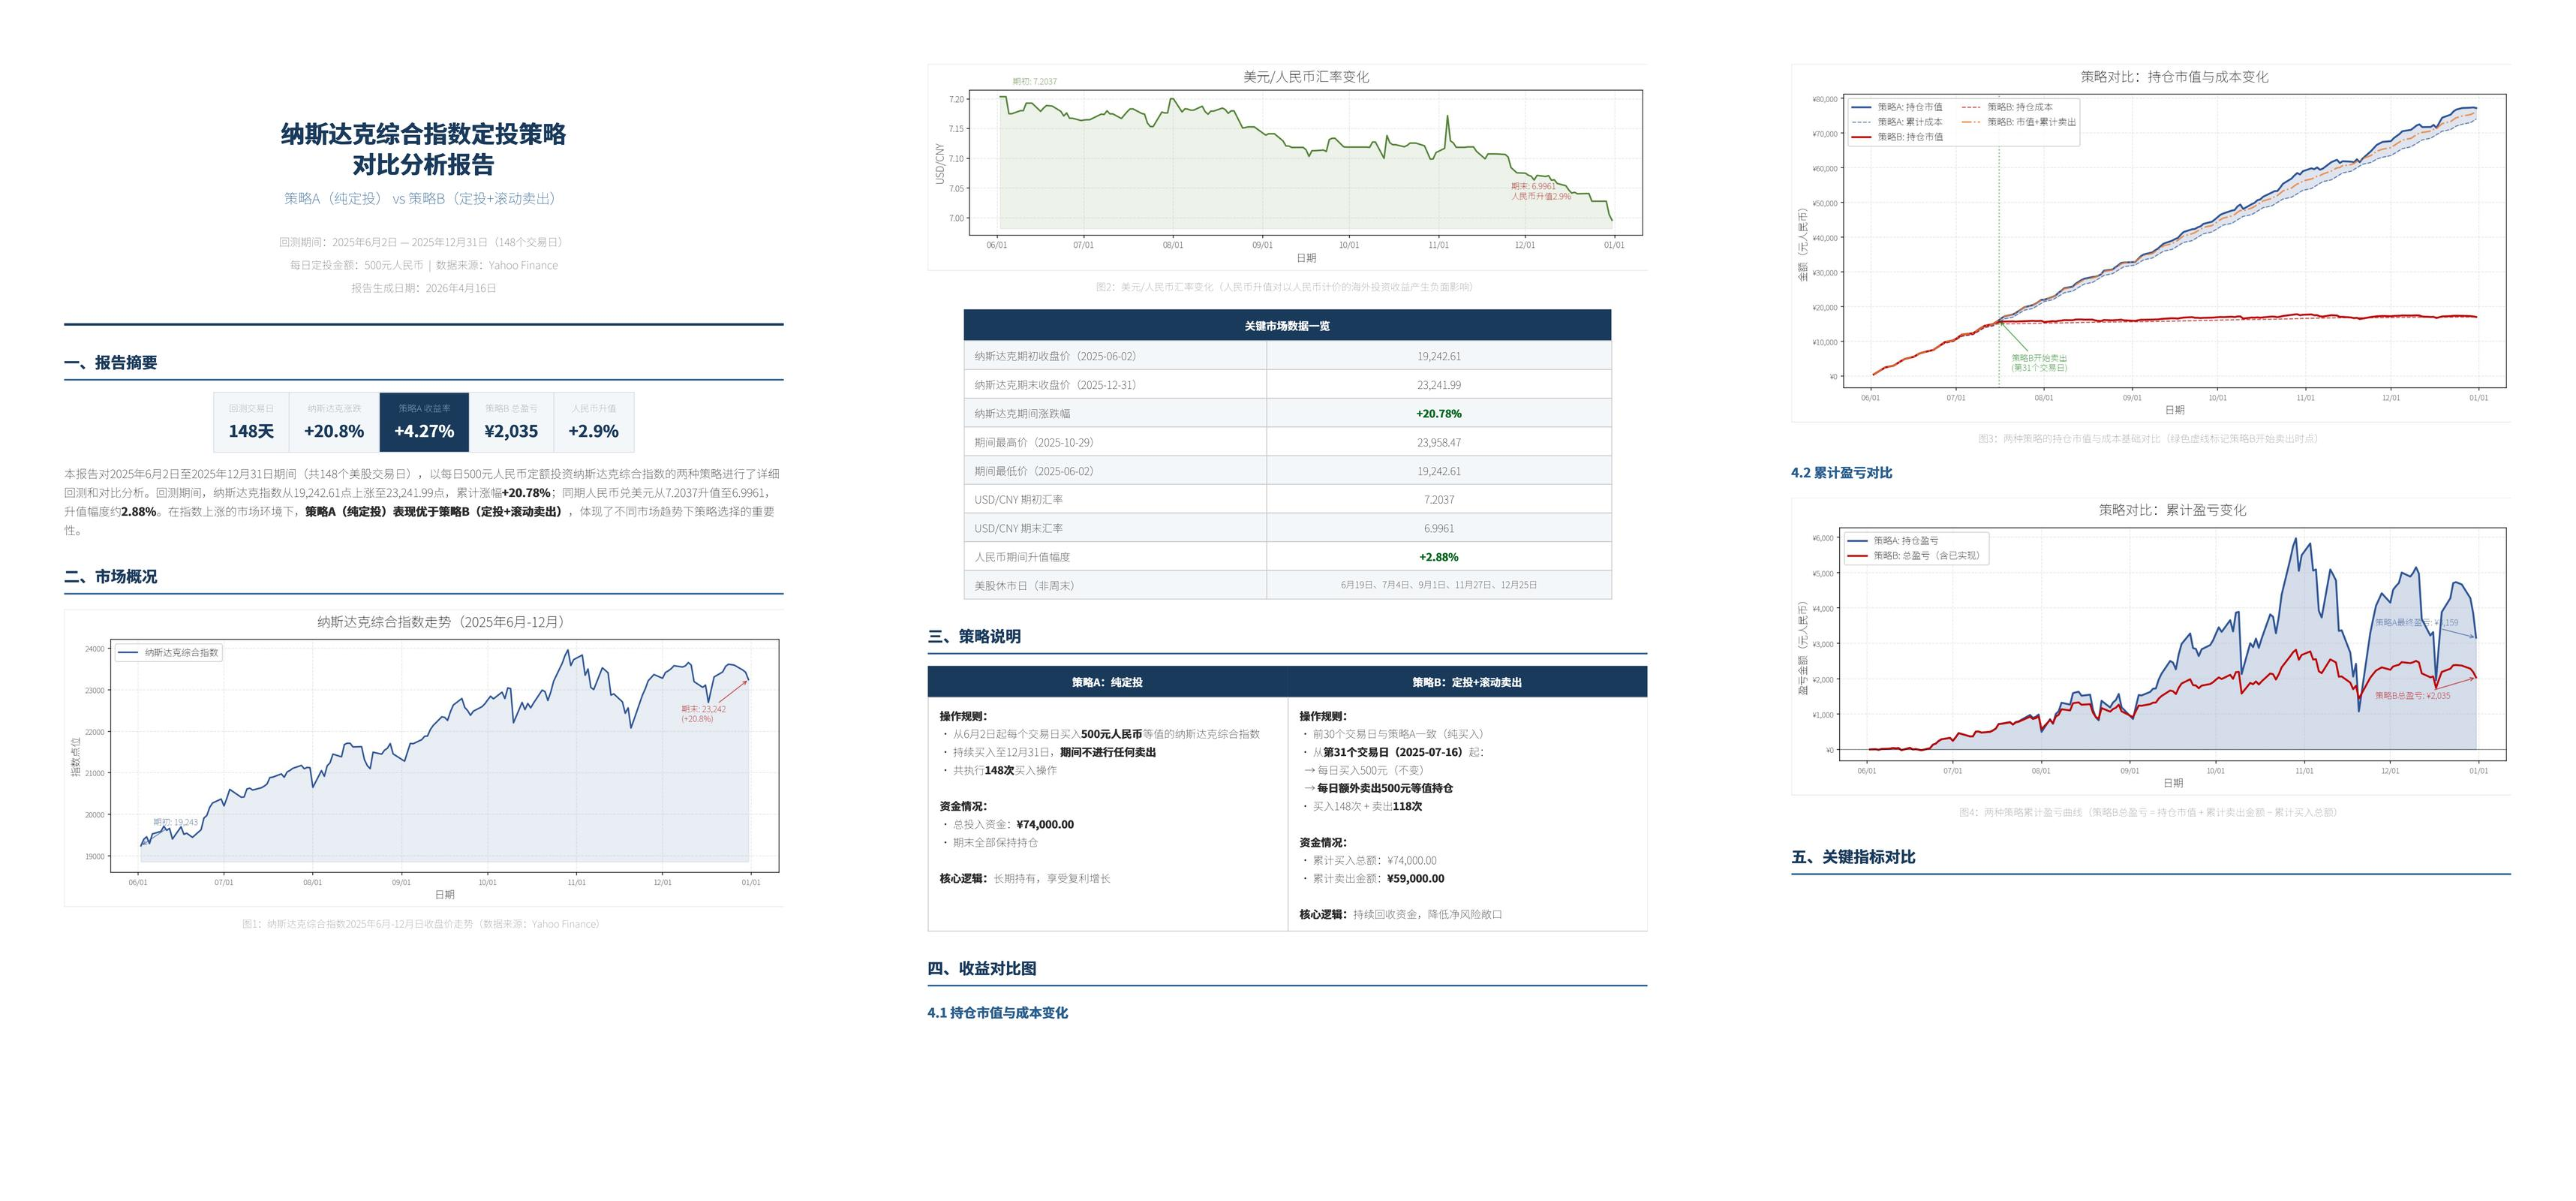
\includegraphics[keepaspectratio,alt={image}]{images_hi/p56-000.jpg}}

图 14 \textbar{} 需要比较纳斯达克两种定投策略的任务输出示例。

\pandocbounded{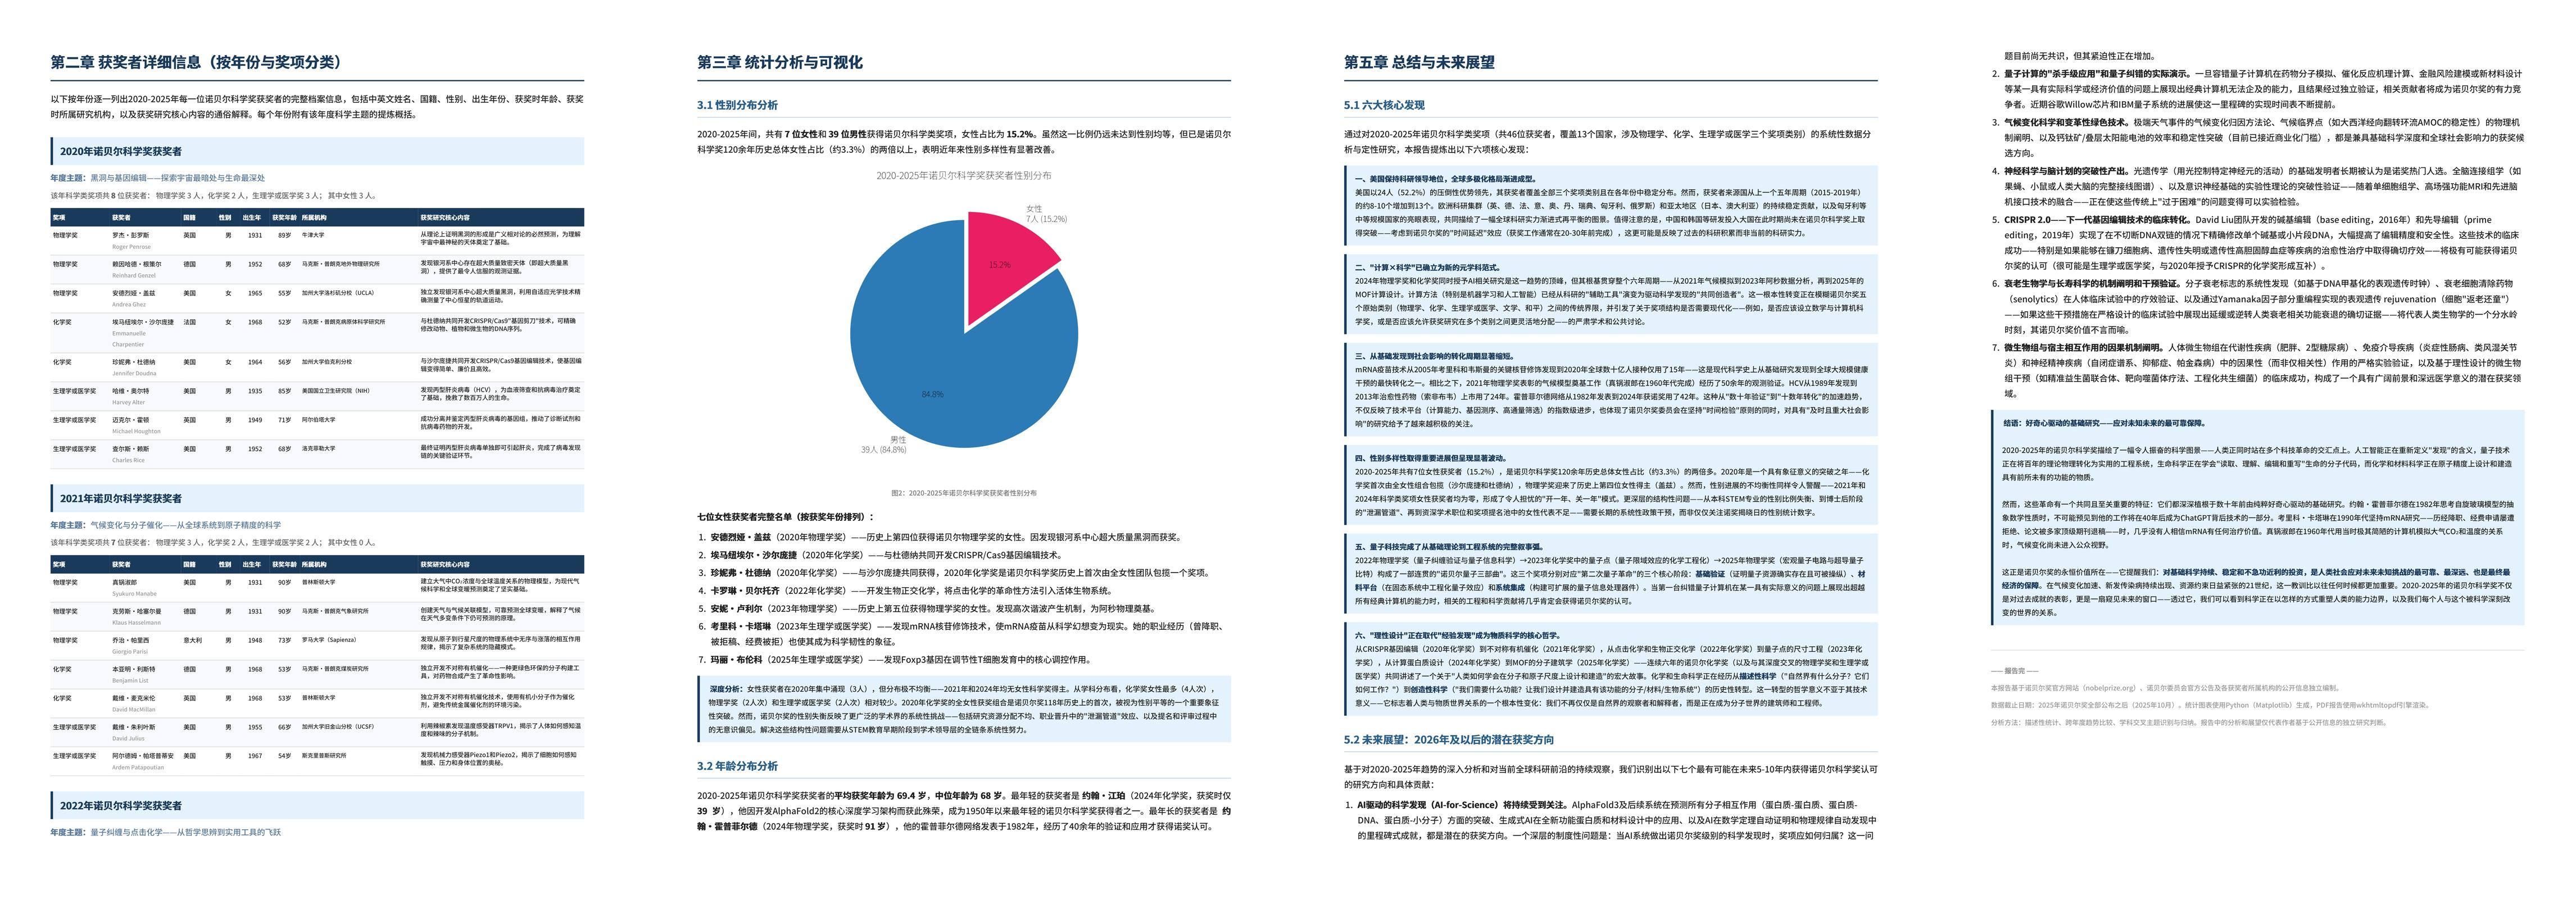
\includegraphics[keepaspectratio,alt={image}]{images_hi/p56-001.jpg}}

图 15 \textbar{} 需要调研 2020-2025 年诺贝尔科学奖并生成分析型 PDF 报告的任务输出示例。

表 12 \textbar{} DeepSeek-V4-Pro 与 Gemini-3.1-Pro 在中文功能性写作上的对比分析。

{\def\LTcaptype{none} % do not increment counter
\begin{longtable}[]{@{}lllllllll@{}}
\toprule\noalign{}
\endhead
\bottomrule\noalign{}
\endlastfoot
\multirow{2}{*}{Category} & \multirow{2}{*}{Subcategory} &
\multirow{2}{*}{\#} & \multicolumn{6}{l@{}}{%
Internal Evaluation (内部综合评估)} \\
& & & DS win & Gem win & Tie & DS\% & Gem\% & Tie\% \\
\multirow{10}{*}{Business Writing (办公文本)} & Report (报告) & 527 &
350 & 162 & 15 & 66.41 & 30.74 & 2.85 \\
& Proposal (方案策划) & 291 & 181 & 103 & 7 & 62.20 & 35.40 & 2.41 \\
& Education (教育培训) & 159 & 100 & 56 & 3 & 62.89 & 35.22 & 1.89 \\
& Email \& Letter (邮件书信) & 146 & 107 & 37 & 2 & 73.29 & 25.34 &
1.37 \\
& Notice (通知公告) & 72 & 43 & 24 & 5 & 59.72 & 33.33 & 6.94 \\
& Professional (专业文本) & 63 & 34 & 27 & 2 & 53.97 & 42.86 & 3.17 \\
& Recruitment (招聘求职) & 42 & 27 & 15 & 0 & 64.29 & 35.71 & 0.00 \\
& Technical (技术文本) & 29 & 22 & 7 & 0 & 75.86 & 24.14 & 0.00 \\
& Review (介绍评价) & 20 & 15 & 5 & 0 & 75.00 & 25.00 & 0.00 \\
& Subtotal (小计) & 1349 & 879 & 436 & 34 & 65.16 & 32.32 & 2.52 \\
\multirow{9}{*}{Media Writing (媒体文本)} & Social Media (社交媒体文案)
& 267 & 156 & 101 & 10 & 58.43 & 37.83 & 3.75 \\
& Ad Copy (广告商品文案) & 214 & 109 & 98 & 7 & 50.93 & 45.79 & 3.27 \\
& Long-form Content (内容平台长文) & 99 & 71 & 25 & 3 & 71.72 & 25.25 &
3.03 \\
& News Report (新闻报道) & 51 & 27 & 22 & 2 & 52.94 & 43.14 & 3.92 \\
& Advertorial (营销软文) & 17 & 12 & 4 & 1 & 70.59 & 23.53 & 5.88 \\
& Headline (标题) & 11 & 7 & 4 & 0 & 63.64 & 36.36 & 0.00 \\
& Narration Script (口播文案) & 4 & 2 & 1 & 1 & 50.00 & 25.00 & 25.00 \\
& Comment (评论) & 3 & 2 & 1 & 0 & 66.67 & 33.33 & 0.00 \\
& Subtotal (小计) & 666 & 386 & 256 & 24 & 57.96 & 38.44 & 3.60 \\
\multirow{6}{*}{Everyday Writing (生活文本)} & Congratulatory (祝贺文本)
& 101 & 54 & 41 & 6 & 53.47 & 40.59 & 5.94 \\
& Communication (沟通回复) & 100 & 71 & 26 & 3 & 71.00 & 26.00 & 3.00 \\
& Reflection (心得感想) & 90 & 68 & 17 & 5 & 75.56 & 18.89 & 5.56 \\
& Review (介绍评价) & 55 & 44 & 9 & 2 & 80.00 & 16.36 & 3.64 \\
& Comment (评论) & 44 & 34 & 8 & 2 & 77.27 & 18.18 & 4.55 \\
& Subtotal (小计) & 390 & 271 & 101 & 18 & 69.49 & 25.90 & 4.62 \\
\multirow{6}{*}{Oral Writing (口头文本)} & Speech (发言稿) & 226 & 135 &
85 & 6 & 59.73 & 37.61 & 2.65 \\
& Narration Script (口播文案) & 51 & 25 & 23 & 3 & 49.02 & 45.10 &
5.88 \\
& Sales Script (话术) & 31 & 22 & 6 & 3 & 70.97 & 19.35 & 9.68 \\
& Dialogue (对话文本) & 10 & 4 & 6 & 0 & 40.00 & 60.00 & 0.00 \\
& Congratulatory (祝贺文本) & 1 & 1 & 0 & 0 & 100.00 & 0.00 & 0.00 \\
& Subtotal (小计) & 319 & 187 & 120 & 12 & 58.62 & 37.62 & 3.76 \\
\multirow{6}{*}{Official Document (公文文本)} & Administrative Doc
(事务文书) & 117 & 60 & 53 & 4 & 51.28 & 45.30 & 3.42 \\
& Personal Doc (个人文书) & 73 & 45 & 27 & 1 & 61.64 & 36.99 & 1.37 \\
& Government Doc (行政公文) & 34 & 19 & 14 & 1 & 55.88 & 41.18 & 2.94 \\
& Speech (发言稿) & 3 & 1 & 2 & 0 & 33.33 & 66.67 & 0.00 \\
& Essay Writing (申论写作) & 3 & 1 & 1 & 1 & 33.33 & 33.33 & 33.33 \\
& Subtotal (小计) & 230 & 126 & 97 & 7 & 54.78 & 42.17 & 3.04 \\
\multirow{5}{*}{Academic Writing (学术文本)} & Research Paper (学术论文)
& 104 & 67 & 32 & 5 & 64.42 & 30.77 & 4.81 \\
& Coursework (课程作业) & 90 & 53 & 35 & 2 & 58.89 & 38.89 & 2.22 \\
& Academic Support (学术辅助) & 15 & 11 & 3 & 1 & 73.33 & 20.00 &
6.67 \\
& Science Outreach (专业科普) & 7 & 6 & 1 & 0 & 85.71 & 14.29 & 0.00 \\
& Subtotal (小计) & 216 & 137 & 71 & 8 & 63.43 & 32.87 & 3.70 \\
Total (总计) & & 3170 & 1986 & 1081 & 103 & 62.65 & 34.10 & 3.25 \\
\end{longtable}
}

表 13 \textbar{} DeepSeek-V4-Pro 与 Gemini-3.1-Pro 在中文创意写作上的对比分析。

{\def\LTcaptype{none} % do not increment counter
\begin{longtable}[]{@{}llllllllllllll@{}}
\toprule\noalign{}
\endhead
\bottomrule\noalign{}
\endlastfoot
\multirow{2}{*}{Subcategory (文体)} & \multirow{2}{*}{\#} &
\multicolumn{6}{l}{%
Instruction Following(指令遵循)} & \multicolumn{6}{l@{}}{%
Writing Quality (写作质量)} \\
& & DS & Gem & Tie & DS\% & Gem\% & Tie\% & DS & Gem & Tie & DS\% &
Gem\% & Tie\% \\
Fiction (小说故事) & 836 & 504 & 323 & 5 & 60.58 & 38.82 & 0.60 & 672 &
157 & 3 & 80.77 & 18.87 & 0.36 \\
General Fiction (泛小说故事) & 662 & 368 & 290 & 3 & 55.67 & 43.87 &
0.45 & 467 & 194 & 0 & 70.65 & 29.35 & 0.00 \\
Fan Fiction (同人文) & 410 & 253 & 150 & 3 & 62.32 & 36.95 & 0.74 & 338
& 67 & 1 & 83.25 & 16.50 & 0.25 \\
General Fan Fic. (泛同人文) & 202 & 111 & 90 & 1 & 54.95 & 44.55 & 0.50
& 161 & 40 & 1 & 79.70 & 19.80 & 0.50 \\
Narrative (记叙文) & 171 & 115 & 54 & 2 & 67.25 & 31.58 & 1.17 & 141 &
30 & 0 & 82.46 & 17.54 & 0.00 \\
General Prose (泛散文) & 124 & 83 & 40 & 1 & 66.94 & 32.26 & 0.81 & 88 &
36 & 0 & 70.97 & 29.03 & 0.00 \\
Prose (散文) & 112 & 74 & 38 & 0 & 66.07 & 33.93 & 0.00 & 92 & 20 & 0 &
82.14 & 17.86 & 0.00 \\
Writing Style (文笔) & 112 & 81 & 31 & 0 & 72.32 & 27.68 & 0.00 & 86 &
26 & 0 & 76.79 & 23.21 & 0.00 \\
Classical Poetry (古诗文) & 48 & 24 & 24 & 0 & 50.00 & 50.00 & 0.00 & 39
& 9 & 0 & 81.25 & 18.75 & 0.00 \\
Modern Poetry (现代诗) & 43 & 23 & 20 & 0 & 53.49 & 46.51 & 0.00 & 32 &
11 & 0 & 74.42 & 25.58 & 0.00 \\
Lyrics (歌词) & 30 & 8 & 22 & 0 & 26.67 & 73.33 & 0.00 & 16 & 14 & 0 &
53.33 & 46.67 & 0.00 \\
Literary Appreciation (赏析) & 27 & 20 & 7 & 0 & 74.07 & 25.93 & 0.00 &
18 & 9 & 0 & 66.67 & 33.33 & 0.00 \\
General Argument. (泛议论文) & 24 & 15 & 9 & 0 & 62.50 & 37.50 & 0.00 &
17 & 7 & 0 & 70.83 & 29.17 & 0.00 \\
General Narrative (泛记叙文) & 23 & 11 & 12 & 0 & 47.83 & 52.17 & 0.00 &
15 & 8 & 0 & 65.22 & 34.78 & 0.00 \\
General Classical (泛古文诗歌) & 9 & 5 & 4 & 0 & 55.56 & 44.44 & 0.00 &
5 & 4 & 0 & 55.56 & 44.44 & 0.00 \\
Creative Writing (创意写作) & 6 & 2 & 4 & 0 & 33.33 & 66.67 & 0.00 & 4 &
2 & 0 & 66.67 & 33.33 & 0.00 \\
Argumentative (议论文) & 5 & 5 & 0 & 0 & 100.00 & 0.00 & 0.00 & 5 & 0 &
0 & 100.00 & 0.00 & 0.00 \\
General Mod. Poetry (泛现代诗) & 2 & 1 & 1 & 0 & 50.00 & 50.00 & 0.00 &
2 & 0 & 0 & 100.00 & 0.00 & 0.00 \\
Total (总计) & 2837 & 1703 & 1119 & 15 & 60.03 & 39.44 & 0.53 & 2198 &
634 & 5 & 77.48 & 22.35 & 0.18 \\
\end{longtable}
}

表 14 \textbar{} DeepSeek-V4-Pro 与 Claude-Opus-4.5 在复杂指令遵循与多轮写作上的对比。

{\def\LTcaptype{none} % do not increment counter
\begin{longtable}[]{@{}llllllll@{}}
\toprule\noalign{}
\endhead
\bottomrule\noalign{}
\endlastfoot
\multirow{2}{*}{Category} & \multirow{2}{*}{\#} &
\multicolumn{6}{l@{}}{%
Internal Evaluation (内部综合评估)} \\
& & DS & Opus & Tie & DS\% & Opus\% & Tie\% \\
Complex Inst. Following (复杂指令跟随) & 49 & 23 & 26 & 0 & 46.9\% &
53.1\% & 0.0\% \\
Multi-Turn Writing (多轮写作) & 147 & 67 & 76 & 4 & 45.6\% & 51.7\% &
2.7\% \\
Total (总计) & 196 & 90 & 102 & 4 & 45.9\% & 52.0\% & 2.0\% \\
\end{longtable}
}
